%% For submission and review of your manuscript please change the
%% command to \documentclass[manuscript, screen, review]{acmart}.
%%
%% When submitting camera ready or to TAPS, please change the command
%% to \documentclass[sigconf]{acmart} or whichever template is required
%% for your publication.
%% 
\documentclass[acmsmall]{acmart}
%\documentclass[sigconf,anonymous]{acmart}
% \documentclass[sigconf,review,anonymous,10pt]{acmart}
% \documentclass[acmsmall,anonymous,review]{acmart}
\usepackage{soul}
\usepackage{enumitem}
\usepackage{mathtools}
\usepackage{empheq}
\usepackage{graphicx}
\usepackage{epstopdf}
\usepackage{svg}
\usepackage[normalem]{ulem}
% TODO:
\setcopyright{acmlicensed}
\copyrightyear{2025}
\acmYear{2025}
\acmDOI{XXXXXXX.XXXXXXX}
% After the abstract deadline, DOI will be emailed to the author

% NOTE: Control Option
\renewcommand\footnotetextcopyrightpermission[1]{}
\settopmatter{printacmref=false} %remove ACM reference format

%% These commands are for a PROCEEDINGS abstract or paper.

%\acmConference[APNet'25]{9th Asia-Pacific Workshop on Networking}{August 7--8, 2025}{Shanghai, China}
\acmConference{}
%%  Uncomment \acmBooktitle if the title of the proceedings is different
%%  from ``Proceedings of ...''!
%%
%%\acmBooktitle{Woodstock '18: ACM Symposium on Neural Gaze Detection,
%%  June 03--05, 2018, Woodstock, NY}
\acmISBN{}

% NOTE: 
\newcommand{\zyu}[1]{\textcolor{blue}{#1}}
\newcommand{\wcb}[1]{\textcolor{red}{#1}}

\newcommand{\wcbinfo}[1]{\textcolor[HTML]{8831cc}{#1}}
\newcommand{\wcbwarn}[1]{\textcolor[HTML]{e91e2c}{#1}}
\newcommand{\wcbobjchange}[1]{\textcolor[HTML]{f06b06}{#1}}

\graphicspath{{figures/}}
\usepackage{subfigure}
\usepackage{xspace}
\newcommand{\ours}{\textsc{SWOT}\xspace}
\newcommand{\newapproach}{intra-collective reconfiguration\xspace}
\newcommand{\newapproachst}{intra-collective\xspace}
\newcommand{\strawman}{Strawman-ICR\xspace}
% intra-iteration reconfiguration -> Intra-collective Reconfiguration
% Strawman-IIR -> Strawman-ICR
\newcommand{\us}{\textmu{}s\xspace}

%% ------------------------------------------------------- %%
\begin{document}
%% ----------------------% Title %----------------------- %%
% \title[Improving Optical Network Scalability in CC Via Reconfiguration-Communication Overlap]{Improving Optical Network Scalability in Collective Communication Via Reconfiguration-Communication Overlap}
\title{Utility-Guided Agent Orchestration for Efficient LLM Tool Use}
%% ---------------------% Authors %---------------------- %%
%% Of note is the shared affiliation of the first two authors, and the
%% "authornote" and "authornotemark" commands
%% used to denote shared contribution to the research.
\newcommand{\ustc}{University of Science and Technology of China}

\author{Boyan Liu}
\email{lby24011252@mail.ustc.edu.cn}
\affiliation{
  \institution{\ustc}
  \city{Hefei}
  \state{Anhui}
  \country{China}
}

\author{Gongming Zhao}
\email{gmzhao@ustc.edu.cn}
%\orcid{} 
\affiliation{
  \institution{\ustc}
  \city{Hefei}
  \state{Anhui}
  \country{China}
}

\author{Hongli Xu}
\email{xuhongli@ustc.edu.cn}
%\orcid{} 
\affiliation{
  \institution{\ustc}
  \city{Hefei}
  \state{Anhui}
  \country{China}
}
%% By default, the full list of authors will be used in the page
%% headers. Often, this list is too long, and will overlap
%% other information printed in the page headers. This command allows
%% the author to define a more concise list
%% of authors' names for this purpose.
%\renewcommand{\shortauthors}{Wu et al.}

%% ---------------------% Abstract %---------------------- %%
\begin{abstract}
Tool-using large language model (LLM) agents often face a fundamental tension between answer quality and execution cost. Fixed workflows are stable but inflexible, while free-form multi-step reasoning methods such as ReAct may improve task performance at the expense of excessive tool calls, longer trajectories, higher token consumption, and increased latency. In this paper, we study \emph{agent orchestration} as an explicit decision problem rather than leaving it entirely to prompt-level behavior. We propose a utility-guided orchestration policy that selects among actions such as \texttt{respond}, \texttt{retrieve}, \texttt{tool\_call}, \texttt{verify}, and \texttt{stop} by balancing estimated gain, step cost, uncertainty, and redundancy. Our goal is not to claim universally best task performance, but to provide a controllable and analyzable policy framework for studying quality--cost trade-offs in tool-using LLM agents. Experiments across direct answering, threshold control, fixed workflows, ReAct, and several policy variants show that explicit orchestration signals substantially affect agent behavior. Additional analyses on cost definitions, workflow fairness, and redundancy control further demonstrate that lightweight utility design can provide a defensible and practical mechanism for agent control.
\end{abstract}

%% A "teaser" image appears between the author and affiliation
%% information and the body of the document, and typically spans the
%% page.
%\begin{teaserfigure}
%  \includegraphics[width=\textwidth]{figures/sampleteaser}
%  \caption{Seattle Mariners at Spring Training, 2010.}
%  \Description{Enjoying the baseball game from the third-base
%  seats. Ichiro Suzuki preparing to bat.}
%  \label{fig:teaser}
%\end{teaserfigure}

% TODO: 
%\received{20 February 2007}
%\received[revised]{12 March 2009}
%\received[accepted]{5 June 2009}

\maketitle
%% ---------------------% Contents %---------------------- %%
\section{Introduction}

Large language model (LLM) agents are increasingly equipped with external tools such as search engines, retrievers, calculators, and code interfaces. Such tool-using agents have shown promise in question answering, decision support, and interactive problem solving. However, practical agent systems often suffer from a persistent systems-level problem: better task performance usually requires more reasoning steps, more tool interactions, and longer execution trajectories, which in turn increase token usage and wall-clock latency.

Existing approaches typically fall into two broad categories. The first category uses fixed workflows, where the execution pipeline is manually specified in advance. These methods are stable and predictable, but they are often too rigid to adapt to task difficulty or changing intermediate evidence. The second category uses free-form agent reasoning, such as ReAct-style interaction loops, where the model repeatedly reasons, acts, and observes. These methods are more flexible and often stronger in task quality, but they can also incur unnecessary intermediate steps, repeated tool calls, and inflated execution cost.

This paper focuses on the following question: \emph{can agent behavior be controlled more explicitly, so that the trade-off between answer quality and execution cost becomes more analyzable and more controllable?} Instead of treating orchestration as an implicit consequence of prompting alone, we formulate it as an explicit decision problem. At each step, the agent chooses among actions such as answering directly, retrieving more evidence, invoking a tool, verifying current evidence, or stopping. We instantiate this idea with a utility-guided policy that scores candidate actions using heuristic signals including estimated gain, step cost, uncertainty, and redundancy.

Our contribution is not to propose a fully learned reinforcement learning policy, nor to claim universal superiority over all baselines. Rather, we make three more targeted contributions. First, we provide an explicit orchestration framework for tool-using LLM agents. Second, we analyze how different utility components affect the quality--cost trade-off. Third, we strengthen the empirical discussion through dedicated analyses of cost proxy design, workflow fairness, and redundancy control. These results show that explicit orchestration is a meaningful systems problem in its own right, and that even lightweight utility-guided control can offer useful structure for building more efficient and more interpretable agents.
These results show that explicit orchestration is a meaningful systems problem in its own right, and that even lightweight utility-guided control can offer useful structure for building more efficient and more interpretable agents.

Our implementation and experimental code are publicly available at \url{https://github.com/kagami-kasumi/Utility-Guided-Agent-Orchestration-for-Efficient-LLM-Tool-Use}.

\begin{figure}[t]
\centering
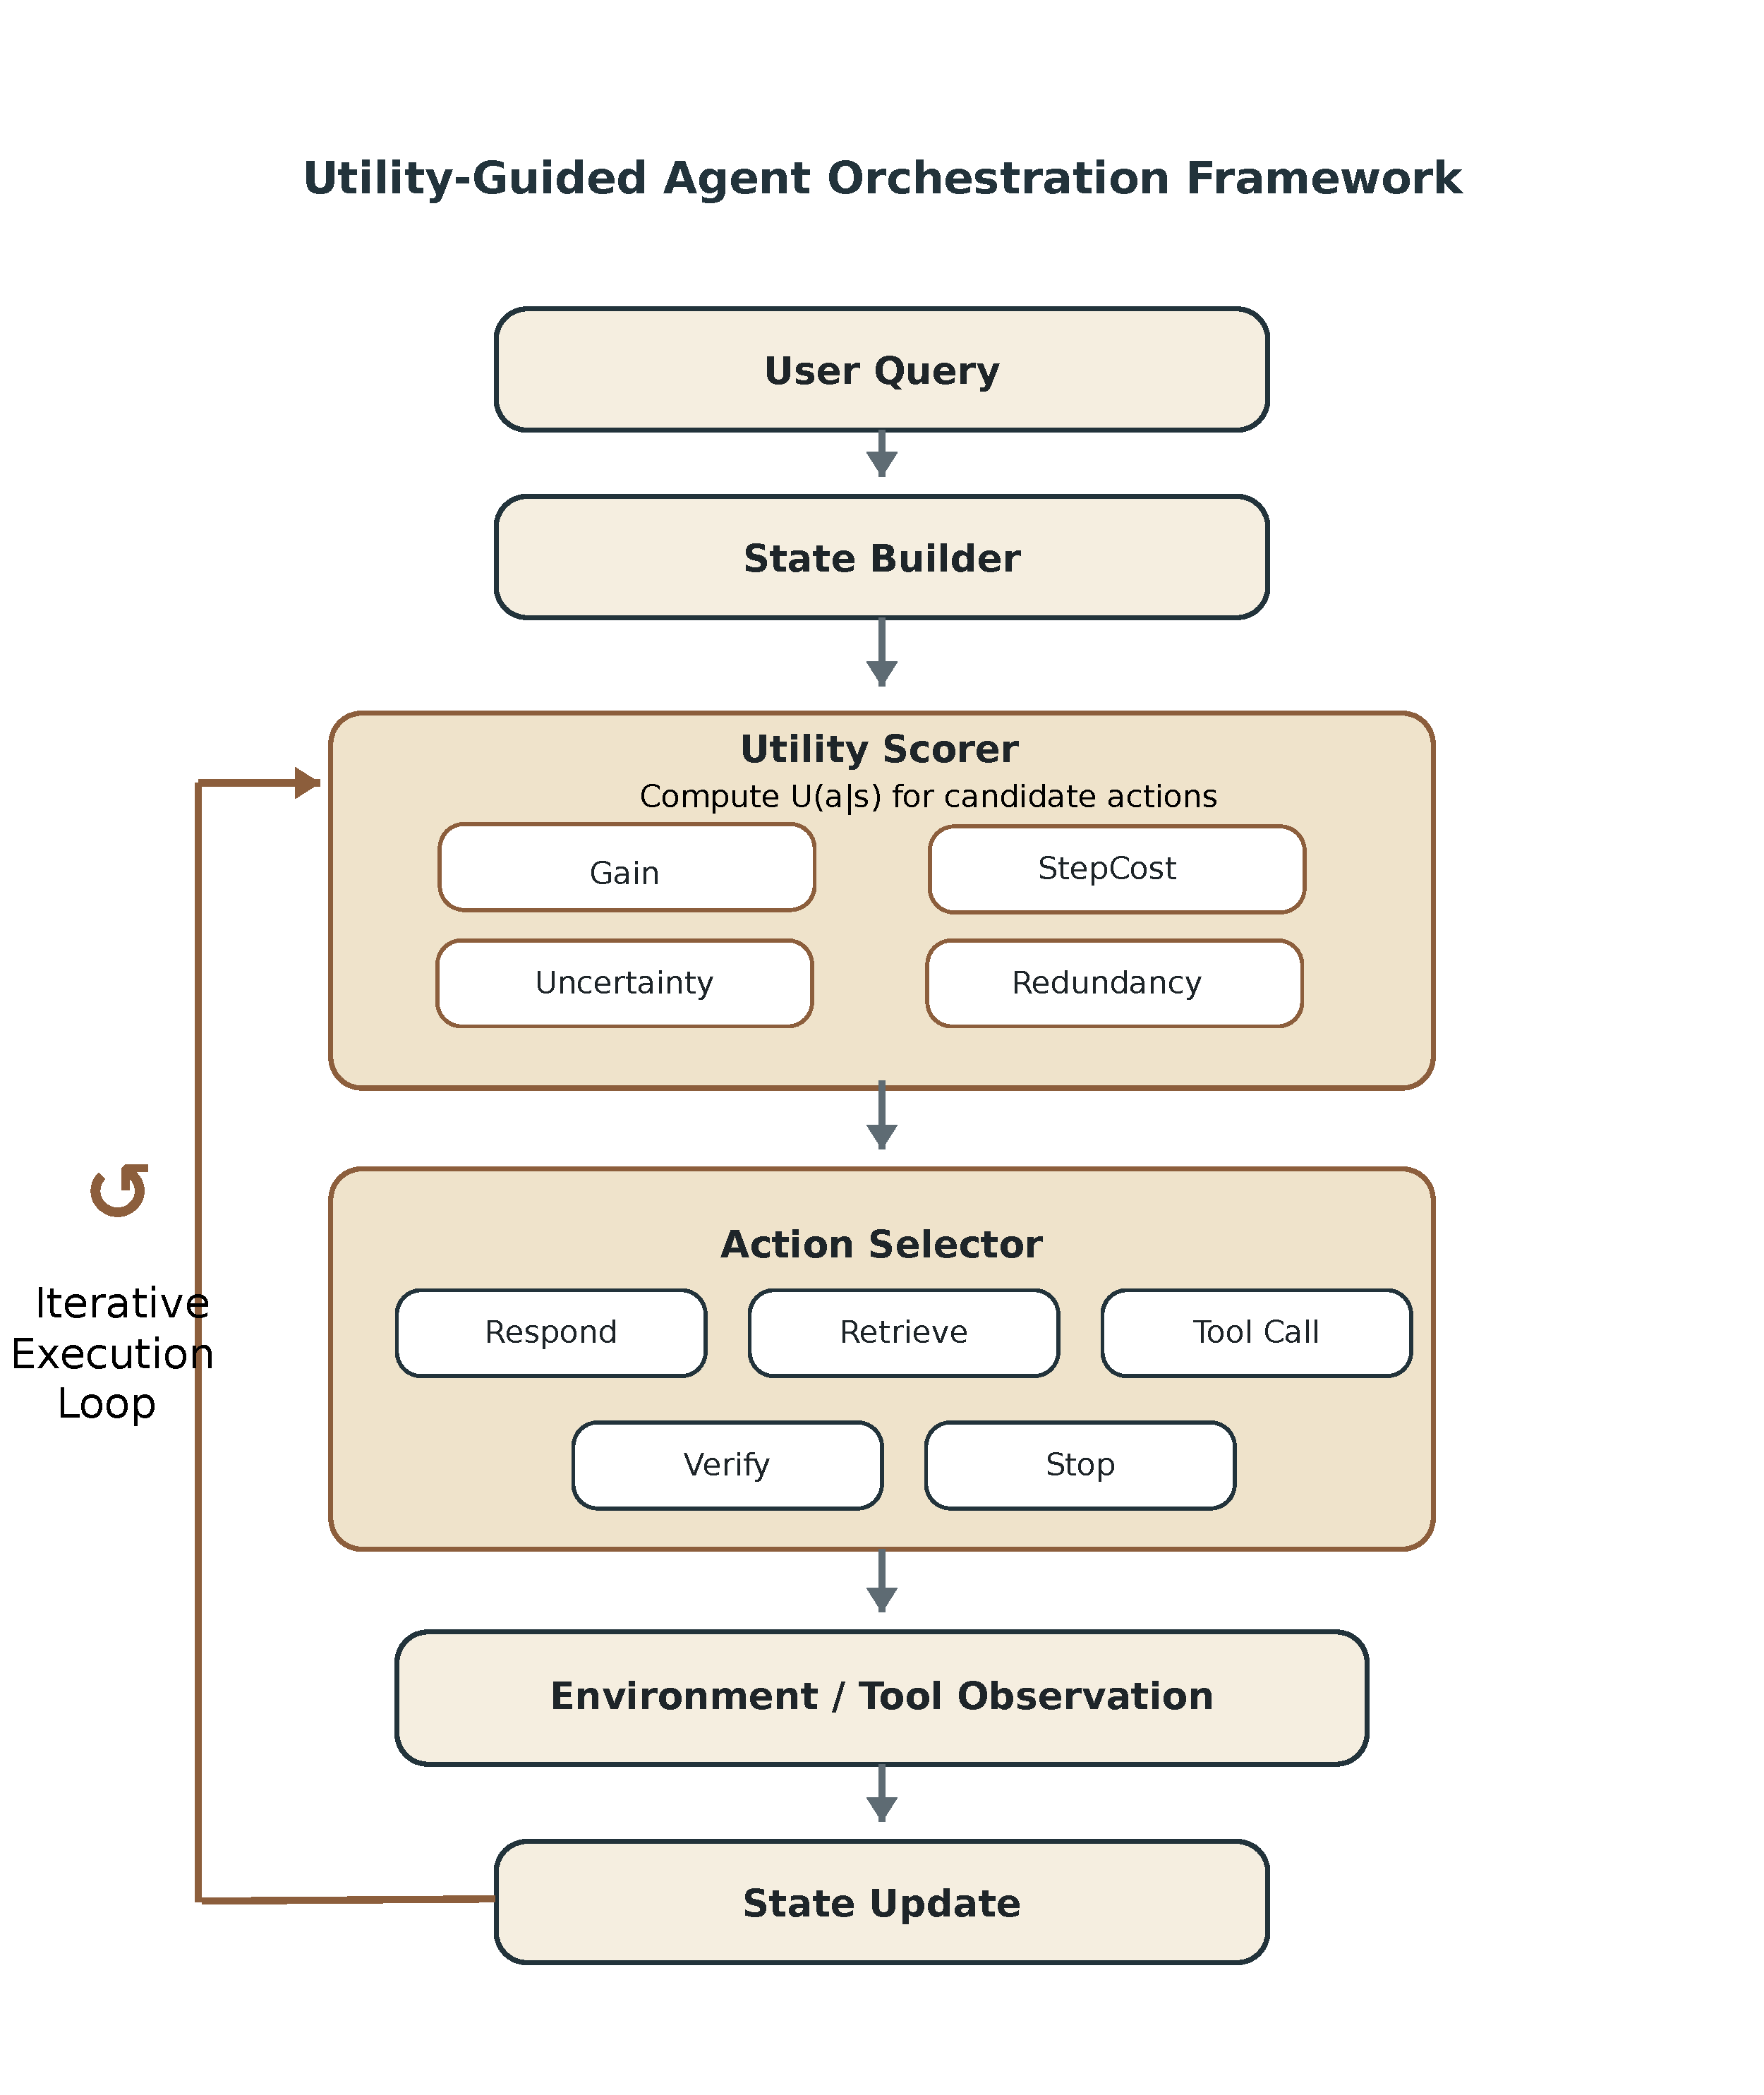
\includegraphics[width=120mm]{figures/overview.pdf}
\caption{
Overview of the proposed utility-guided agent orchestration framework.
At each step, the agent constructs a state representation from the current query, interaction history, and tool observations.
A utility scorer evaluates candidate actions using estimated gain, step cost, uncertainty, and redundancy, and the action selector chooses the highest-utility action.
The process iterates until a stopping condition is met.
}
\label{fig:framework}
\end{figure}
Figure~\ref{fig:framework} illustrates the overall architecture of the proposed framework.

\section{Motivation}

Tool-using LLM agents operate under a persistent tension between \emph{answer quality} and \emph{execution cost}. In principle, additional reasoning, retrieval, and verification steps may improve the final answer. In practice, however, these additional steps are not free: they increase token consumption, wall-clock latency, and trajectory length, and they also enlarge the accumulated prompt context during iterative execution. As a result, practical agent design is not only a reasoning problem, but also a control problem.

This tension is especially visible when contrasting two dominant design patterns. Fixed workflows provide bounded and predictable execution cost, but they are often too rigid to adapt to the difficulty of the current instance or to changing intermediate evidence. On the other hand, free-form multi-step agents, such as ReAct-style systems, can adapt their behavior online, but they may also over-execute. Typical failure modes include repeated retrieval after useful evidence has already been obtained, redundant tool calls with highly similar intent, and continued reasoning even when the marginal value of another step is low. These behaviors do not merely waste computation; they also make agent trajectories harder to interpret and harder to control.

This observation motivates the central perspective of our work: \emph{agent orchestration should be treated as an explicit decision problem rather than an implicit side effect of prompting}. Instead of asking only whether a model can reason or call tools, we ask a more operational question: \emph{when is another action actually worth taking?} Under this view, a tool-using agent should not only know how to retrieve or verify, but should also decide whether retrieval or verification is justified at the current step.

Our goal is therefore different from simply maximizing final answer quality. We aim to make the \emph{quality--cost trade-off} explicit, controllable, and analyzable. This naturally leads to a utility-guided formulation in which candidate actions are evaluated not only by their potential contribution to answer quality, but also by the expected cost of continuing, the current level of uncertainty, and the risk of redundant behavior. Such a formulation turns orchestration into a lightweight control layer between the language model and the external environment.

This perspective is useful for at least three reasons. First, it provides a more interpretable view of multi-step agent execution: the continuation of the trajectory is no longer governed solely by prompt behavior, but also by explicit control signals. Second, it is relevant in budget-sensitive deployments, where excessive reasoning steps directly translate into monetary and latency costs. Third, it matters in context-limited settings, because unnecessary intermediate steps accelerate prompt growth and increase the burden on the context window even when hard truncation is not triggered.

Taken together, these considerations suggest that efficient LLM agents require more than strong reasoning ability or access to external tools. They also require a decision mechanism that regulates \emph{when to continue}, \emph{what action to take next}, and \emph{when to stop}. This is the role played by the orchestration policy studied in this paper.
\section{Related Work}

\subsection{Tool-Using LLM Agents}

Recent progress in large language models (LLMs) has enabled agents to interact with external tools such as search engines, APIs, calculators, and execution environments. A representative line of work studies how language models can interleave reasoning and action during inference. ReAct is a canonical example, showing that alternating between reasoning traces and external actions can improve performance on knowledge-intensive and decision-making tasks~\cite{yao2023react}. Toolformer further demonstrates that language models can learn when and how to invoke tools in a more structured way~\cite{schick2023toolformer}. Gorilla focuses on API-centric tool use and emphasizes the importance of accurate tool selection under realistic interfaces~\cite{patil2023gorilla}. More recent benchmarks and frameworks such as ToolBench further highlight tool-use planning, tool selection, and interaction quality as central concerns for practical LLM agents~\cite{qin2023toolbench}.

These works establish the feasibility and usefulness of tool-using agents, but most of them primarily focus on whether the agent can successfully use tools, rather than how to explicitly control the cost of multi-step behavior. In contrast, our work studies \emph{agent orchestration} as an explicit policy layer that regulates when additional retrieval, tool use, verification, or stopping is worthwhile.

\subsection{Reasoning, Planning, and Self-Improvement}

A second line of work studies how LLMs can reason more effectively through intermediate deliberation or self-improvement. Chain-of-Thought prompting shows that explicit intermediate reasoning can significantly improve complex problem solving~\cite{wei2022chain}. Self-consistency further improves reasoning by sampling multiple chains and aggregating their answers~\cite{wang2023selfconsistency}. Tree of Thoughts generalizes linear reasoning into a more structured search over intermediate thoughts~\cite{yao2023tree}. Program-of-Thoughts prompting instead leverages executable programs to support more reliable reasoning~\cite{chen2023program}. Other works focus on iterative refinement and self-correction, including Self-Refine~\cite{madaan2023selfrefine}, Reflexion~\cite{shinn2023reflexion}, and LATS, which combines language models with tree search over action trajectories~\cite{zhou2024lats}.

While these methods improve reasoning quality, they also tend to increase the number of intermediate steps and the amount of accumulated context. As a result, they do not directly answer the systems-level question of when more reasoning is actually justified. Our work is complementary: rather than proposing a stronger reasoning paradigm, we focus on explicit action selection and stopping decisions under quality--cost trade-offs.

\subsection{Agent Systems, Orchestration, and Multi-Agent Frameworks}

A growing body of work studies LLM agents as systems rather than isolated prompting techniques. AutoGen investigates multi-agent conversation as a mechanism for task decomposition and collaboration~\cite{wu2023autogen}. MetaGPT explores role-based multi-agent software workflows~\cite{hong2024metagpt}. ChatDev similarly models software development as multi-agent communication among role-specialized agents~\cite{qian2024chatdev}. In a different direction, Voyager studies lifelong embodied agents that accumulate skills through iterative exploration~\cite{wang2023voyager}. These works reflect a broader shift from single-shot prompting to agentic systems that involve memory, interaction, coordination, and environment feedback.

However, many existing agent systems still rely heavily on fixed workflows, hand-designed loops, or prompt-driven control. They often leave the orchestration logic implicit, making it difficult to analyze how execution cost arises and how different control signals affect the resulting trajectories. Our work differs in that it makes the orchestration layer explicit and lightweight: instead of proposing a full multi-agent framework or a new interactive environment, we focus on a utility-guided decision mechanism for single-agent tool use.

\subsection{Efficient and Cost-Aware Inference}

Efficiency has become an increasingly important issue in modern LLM systems. Prior work has explored efficient transformer architectures~\cite{tay2022efficient}, adaptive computation mechanisms~\cite{graves2016adaptive}, and early exiting strategies for reducing inference cost~\cite{elbayad2020depth}. Other works study selective prediction, confidence-based routing, or budget-aware computation for neural models~\cite{schuster2022confident,xin2020deebert}. More broadly, recent LLM deployment research has emphasized practical constraints such as token budgets, latency, and context growth.

Compared with this line of research, our work does not propose a new model architecture or a learned adaptive-computation module. Instead, we study efficiency at the orchestration level: the agent explicitly evaluates whether another step is likely to be beneficial, and balances estimated gain against cost-related signals. This makes our approach closer to a lightweight policy layer for tool-using LLM agents, with a focus on analyzing quality--cost trade-offs rather than maximizing task performance alone.

\subsection{Agent Benchmarks and Evaluation}

Recent work has also emphasized the need for realistic evaluation settings for LLM agents. WebShop provides an interactive environment for evaluating multi-step decision making in a web-based shopping setting~\cite{yao2022webshop}. ALFWorld evaluates embodied instruction-following agents in text-based household environments~\cite{shridhar2021alfworld}. ToolBench introduces a large-scale benchmark specifically designed for tool-use agents~\cite{qin2023toolbench}. Other works have pointed out that agent evaluation should consider not only final answer quality, but also trajectory quality, action efficiency, and robustness under realistic execution settings.

Our evaluation perspective is aligned with this broader trend. Rather than measuring only final task quality, we also examine token consumption, wall-clock time, redundancy, and workflow fairness. In this sense, our work contributes to the emerging view that agent quality should be studied together with the computational and behavioral cost of obtaining that quality.
Overall, unlike prior work that primarily emphasizes stronger reasoning, broader tool access, or richer agent frameworks, our work focuses on explicit orchestration as a lightweight decision layer for analyzing and controlling the quality--cost trade-off of tool-using LLM agents.
\section{Design}

\subsection{Problem Formulation}

We study tool-using agent orchestration as a sequential decision problem. Given a user query, the agent interacts with an external environment through a sequence of intermediate steps. At each step $t$, the agent observes a state $s_t$ and must decide whether to answer directly, obtain more external evidence, verify its current information, or terminate execution. The key question is therefore not only \emph{what the model can do}, but also \emph{whether another action is justified at the current stage of execution}.

Formally, we define a compact action space
\[
\mathcal{A} = \{\texttt{respond},\ \texttt{retrieve},\ \texttt{tool\_call},\ \texttt{verify},\ \texttt{stop}\}.
\]
This action space is intentionally lightweight. It is sufficient to capture the main control decisions in a tool-using agent, while remaining simple enough for explicit policy analysis.

\subsection{Agent State}

At step $t$, the agent state $s_t$ includes four categories of information:
\begin{itemize}
    \item the original user query and the current working context,
    \item the interaction history, including prior actions and intermediate reasoning traces,
    \item external observations returned by retrieval or tool calls,
    \item execution-status signals such as step count and budget-related metadata.
\end{itemize}

This state representation is not intended to be a fully learned latent state. Instead, it acts as an explicit control interface between the language model and the environment. Its purpose is to expose enough information for orchestration decisions while keeping the decision layer interpretable.

\subsection{Utility-Guided Action Selection}

To make orchestration explicit, we assign each candidate action $a \in \mathcal{A}$ a utility score
\[
U(a \mid s_t)
=
\mathrm{Gain}(a \mid s_t)
-
\lambda_1 \mathrm{StepCost}(a \mid s_t)
-
\lambda_2 \mathrm{Uncertainty}(a \mid s_t)
-
\lambda_3 \mathrm{Redundancy}(a \mid s_t).
\]

The next action is selected by
\[
a_t^\star = \arg\max_{a \in \mathcal{A}} U(a \mid s_t).
\]

This formulation is deliberately simple. We do not claim that it is an optimal policy in the reinforcement learning sense. Rather, we use it as a structured and analyzable control mechanism for studying how explicit orchestration signals affect multi-step agent behavior.

\subsection{Utility Components}

\paragraph{Estimated Gain.}
$\mathrm{Gain}(a \mid s_t)$ measures the self-estimated marginal value of taking action $a$ at state $s_t$. Intuitively, it captures whether another retrieval, tool call, or verification step is likely to improve the final answer. In our implementation, this term is a heuristic self-estimated signal rather than a calibrated probability.

\paragraph{Step Cost.}
$\mathrm{StepCost}(a \mid s_t)$ is a lightweight normalized proxy for the internal cost of taking one more step. It is designed to discourage unnecessary trajectory expansion. Importantly, this term is not claimed to be an exact substitute for token usage or wall-clock latency. Instead, it acts as an internal control signal whose relationship to real execution cost is examined empirically through token-cost and latency-cost variants. It is therefore best understood as a lightweight control proxy rather than a direct measurement of token or latency cost.

\paragraph{Uncertainty.}
$\mathrm{Uncertainty}(a \mid s_t)$ reflects the agent's self-estimated uncertainty about whether the current evidence is sufficient. Higher uncertainty encourages further evidence gathering or verification, whereas lower uncertainty makes stopping or direct response more plausible. As with estimated gain, this term is heuristic and not calibrated.

\paragraph{Redundancy.}
$\mathrm{Redundancy}(a \mid s_t)$ penalizes repeated or overly similar actions, especially repeated retrieval or tool-use behavior with limited expected novelty. This term is intended to reduce low-value repetition and to compact the execution trajectory. We evaluate both exact-match and semantic variants of this component.

\subsection{Execution Loop and Termination}

Figure~\ref{fig:framework} illustrates the overall execution loop. Starting from the user query, the agent constructs a state representation, computes utility scores for candidate actions, selects the action with the highest utility, and then updates its state based on the resulting observation. This process continues iteratively until one of the following conditions is met:
\begin{itemize}
    \item the selected action is \texttt{stop},
    \item a predefined step budget is exhausted,
    \item or a fallback termination condition is triggered.
\end{itemize}

This termination design is important because stopping is itself part of the control problem. In many free-form agent systems, stopping behavior is only weakly specified by prompts. In our framework, stopping is treated as an explicit action and is therefore subject to the same utility-based decision process as other behaviors.

\subsection{Why Explicit Orchestration?}

The proposed formulation offers two practical benefits. First, it separates task-solving ability from control logic. Rather than embedding all behavior inside a prompt, we expose the orchestration policy as an explicit, inspectable layer. Second, it enables targeted empirical analysis. Because the utility function is decomposed into interpretable components, we can study how cost proxies, uncertainty, redundancy control, and stopping behavior influence the final quality--cost trade-off.

For this reason, the contribution of our framework should not be understood as a fully learned or universally dominant policy. Its value lies in providing a lightweight and defensible mechanism for making multi-step tool use more controllable, more analyzable, and more suitable for cost-sensitive LLM agent settings.
\section{Evaluation}

\subsection{Experimental Setup}

We evaluate all methods on a fixed sample of 200 HotpotQA development examples, using the same base model, the same local BM25 retriever, and the same sampled question set throughout. This controlled setup is important because our goal is not only to compare answer quality, but also to isolate how orchestration policy changes the quality--cost trade-off under matched retrieval and model conditions. We report F1, token consumption, wall-clock time, and the derived efficiency score $F1 / \text{tokens}$.

The compared methods include \texttt{direct} answering, fixed \texttt{workflow} baselines, a \texttt{threshold} controller, \texttt{ReAct}, and our utility-guided \texttt{policy}. For the proposed policy, \texttt{expected\_gain} and \texttt{uncertainty} are treated as LLM self-estimated heuristic signals clipped to $[0,1]$, rather than calibrated probabilities. The default cost term is \texttt{step\_cost}, a normalized step-level proxy. We further validate this choice against token-based and latency-based cost variants in the final-defense experiments.

\subsection{Main Results}

Figures~\ref{fig:main-pareto} and \ref{fig:latency-pareto} summarize the global quality--cost trade-off from both token and latency perspectives, and the exact main-table numbers are reported below.

\begin{figure}[t]
    \centering
    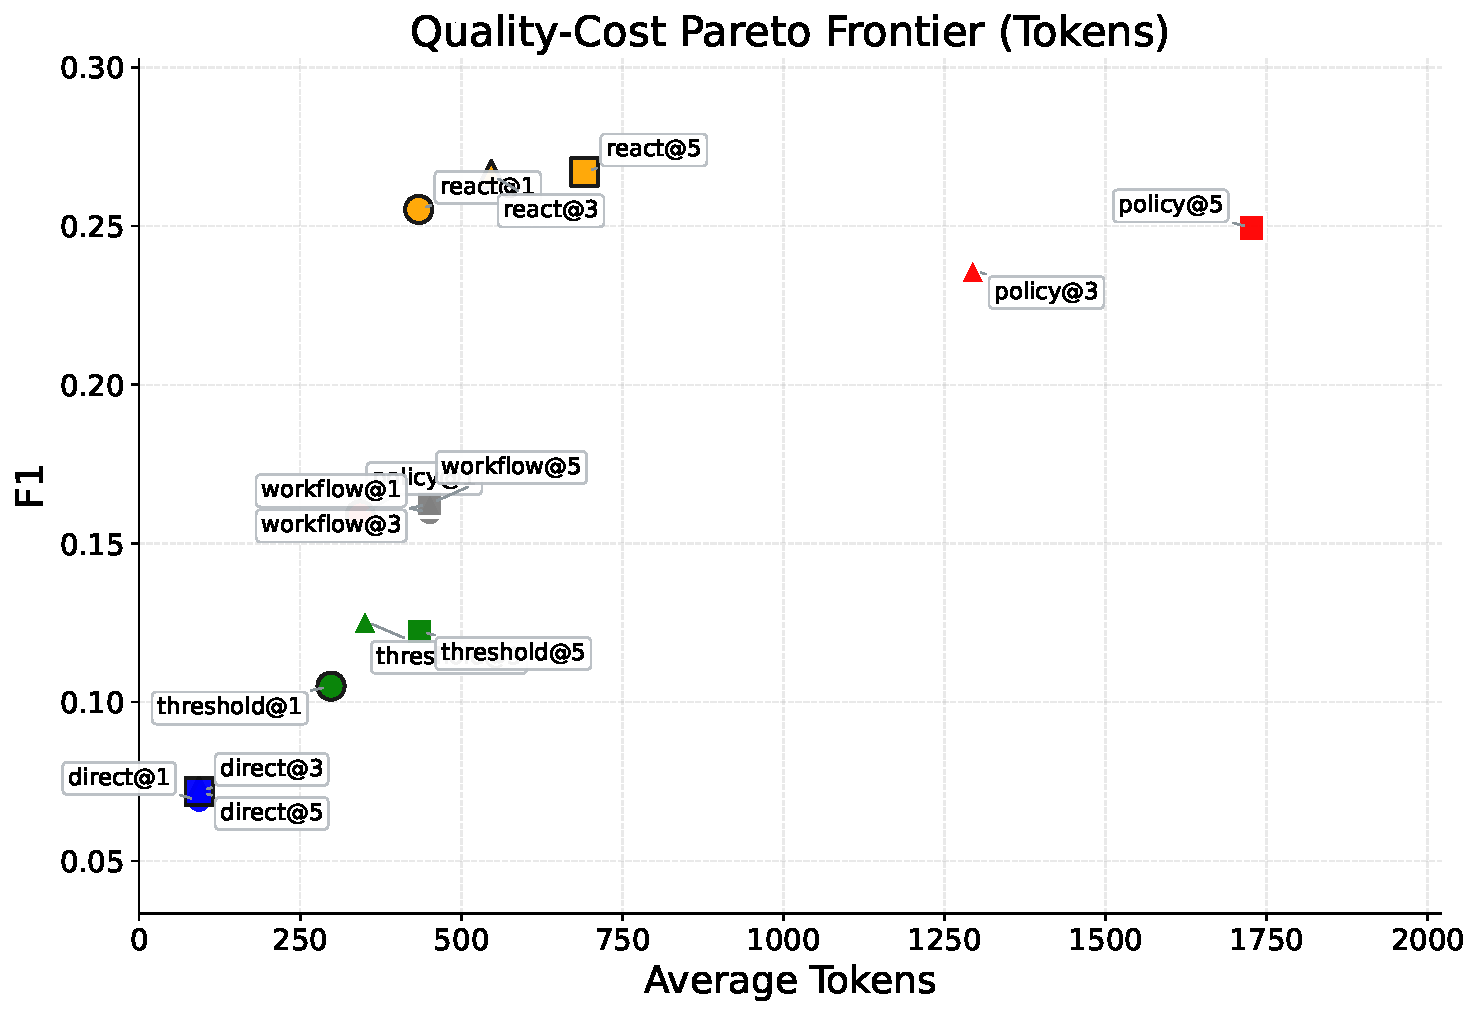
\includegraphics[width=0.82\linewidth]{figures/figure1_pareto_tokens.pdf}
    \caption{Main quality--cost trade-off measured by F1 versus tokens on the shared HotpotQA sample.}
    \label{fig:main-pareto}
\end{figure}

\begin{figure}[t]
    \centering
    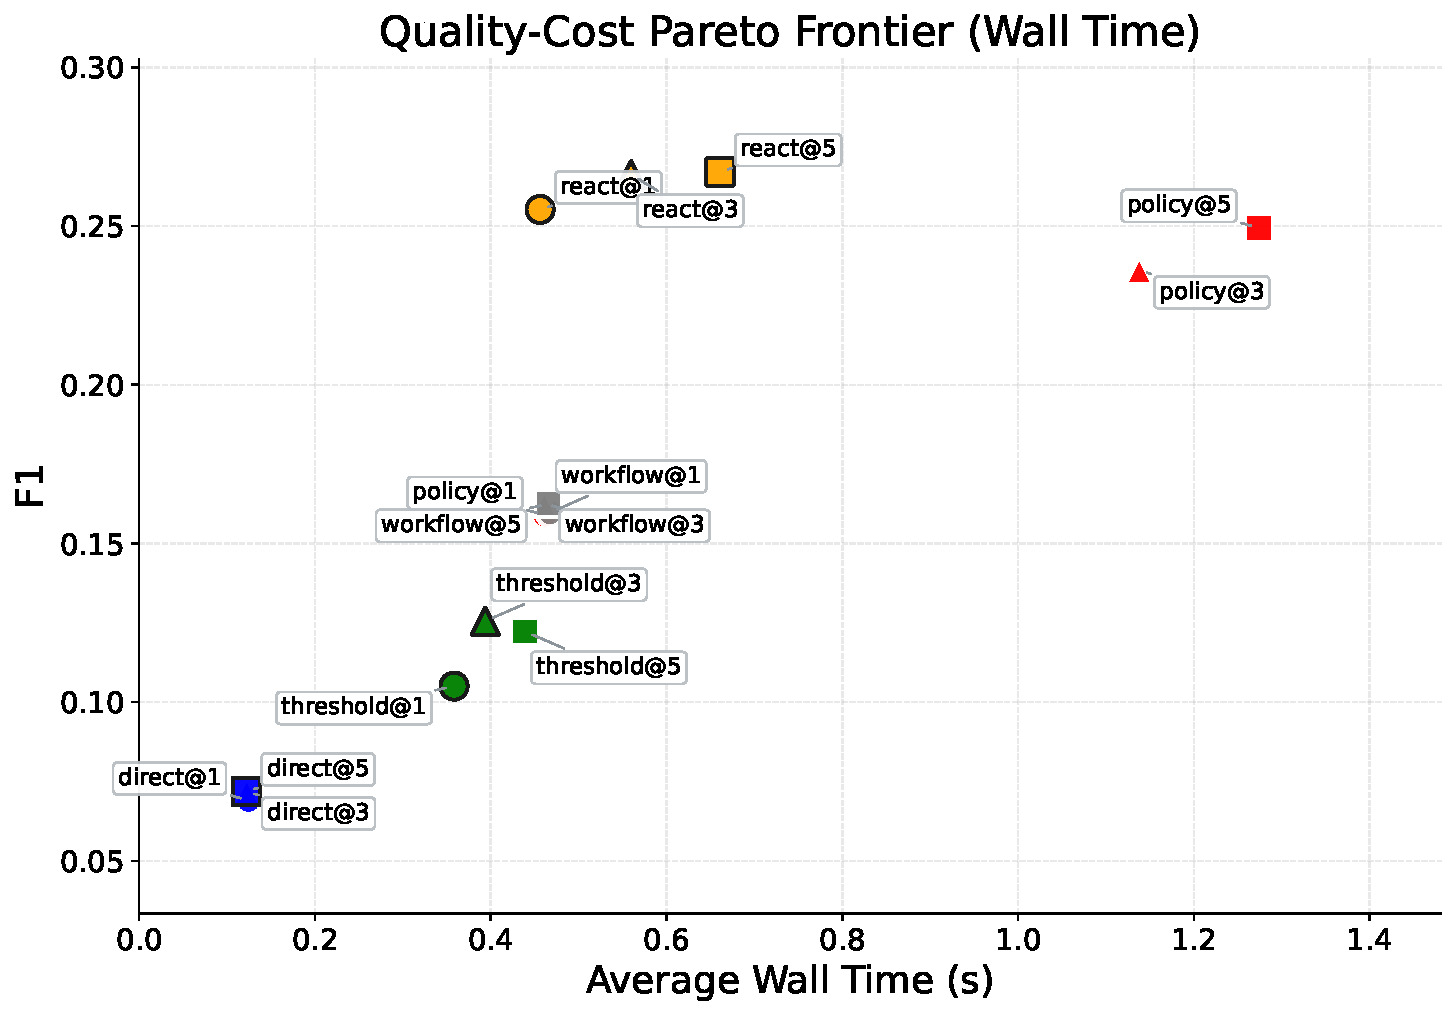
\includegraphics[width=0.82\linewidth]{figures/figure2_pareto_latency.pdf}
    \caption{Main quality--cost trade-off measured by F1 versus wall-clock time. This complements Figure~\ref{fig:main-pareto} by showing the latency-side frontier.}
    \label{fig:latency-pareto}
\end{figure}

\begin{table}[t]
\centering
\small
\caption{Main Results}
\begin{tabular}{lrrrr}
\hline
Method & F1 & Tokens & Wall Time & Efficiency \\
\hline
direct & 0.0719 & 93.0 & 0.122 & 0.000772 \\
workflow (minimal) & 0.1625 & 451.2 & 0.461 & 0.00036 \\
workflow-search-twice & 0.1698 & 514.1 & 0.902 & 0.00033 \\
workflow-search-verify & 0.063 & 1041.2 & 1.617 & 6.1e-05 \\
threshold & 0.1255 & 350.3 & 0.394 & 0.000358 \\
react & 0.2662 & 546.6 & 0.56 & 0.000487 \\
policy (step-cost) & 0.236 & 1294.2 & 1.138 & 0.000182 \\
\hline
\end{tabular}
\end{table}


Several observations are clear. First, \texttt{direct} answering is cheapest but performs poorly ($F1=0.0719$). Second, fixed workflows improve over \texttt{direct}, but remain limited by the lack of adaptive stopping and retrieval choice. Third, \texttt{ReAct} achieves the strongest overall F1 in the main comparison ($0.2662$), confirming the strength of flexible multi-step reasoning. Our \texttt{policy(step\_cost)} reaches $F1=0.2360$ with substantially more explicit control over why it continues, stops, or avoids redundant retrieval.

The evidence supports a more precise conclusion: utility-guided orchestration provides a competitive and interpretable alternative to purely prompt-driven multi-step behavior, and its internal trade-offs can be inspected and modified directly through utility design.

\subsection{Reasoning Depth Analysis}

\begin{figure}[t]
    \centering
    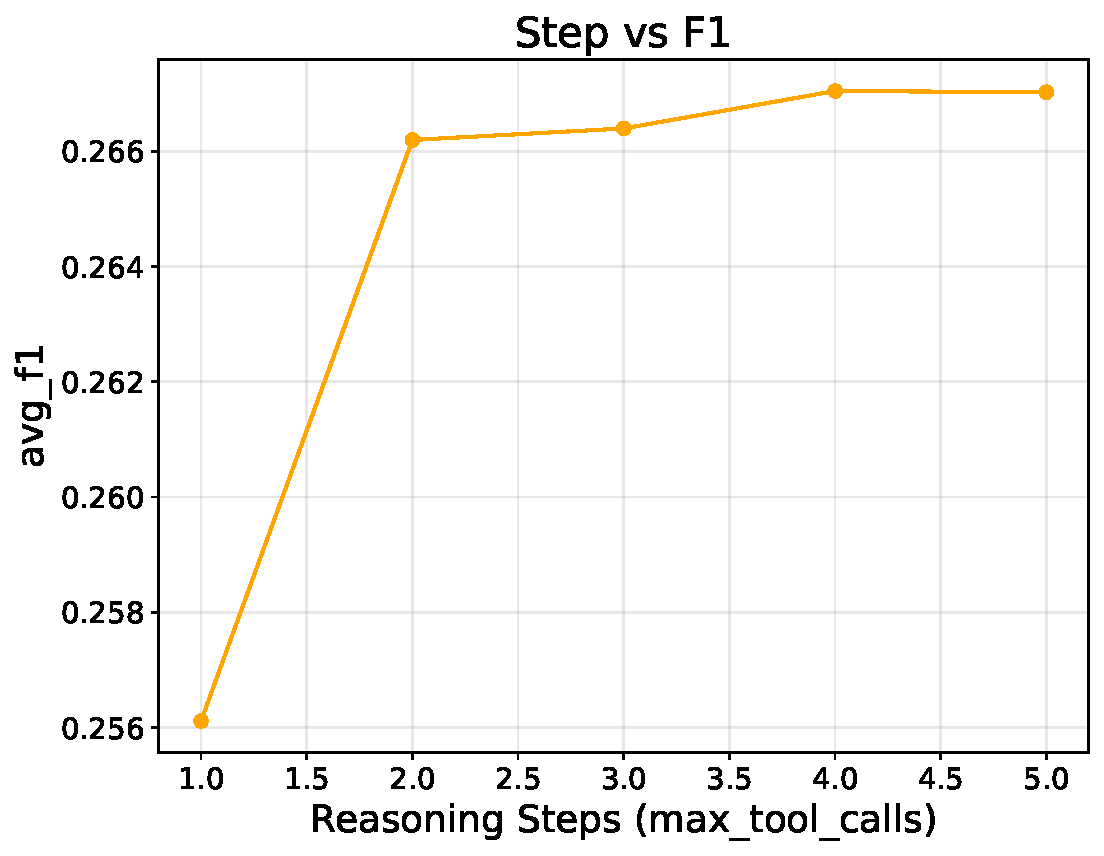
\includegraphics[width=0.88\linewidth]{figures/figure3_step_analysis.pdf}
    \caption{Effect of reasoning depth on answer quality and cost. Increasing the maximum number of reasoning steps improves F1 at first, but also increases token usage and latency, illustrating diminishing marginal returns.}
    \label{fig:step-analysis}
\end{figure}

Figure~\ref{fig:step-analysis} makes the reasoning-depth trade-off explicit. Allowing more reasoning steps initially improves answer quality, but the gains are not linear: token usage and latency rise steadily, while the marginal F1 improvement gradually shrinks. This trend is important for our argument because it shows that orchestration is not only about selecting actions, but also about deciding when additional reasoning is no longer worth the execution cost.

\subsection{Cost Definition Analysis}

\begin{table}[t]
\centering
\small
\caption{Cost Definition Comparison}
\begin{tabular}{lrrrr}
\hline
Method & F1 & Tokens & Wall Time & Efficiency \\
\hline
workflow (minimal) & 0.1625 & 451.2 & 0.461 & 0.00036 \\
react & 0.2662 & 546.6 & 0.56 & 0.000487 \\
threshold & 0.1255 & 350.3 & 0.394 & 0.000358 \\
policy (step-cost) & 0.236 & 1294.2 & 1.138 & 0.000182 \\
policy (token-cost) & 0.2562 & 1308.6 & 1.215 & 0.000196 \\
policy (latency-cost) & 0.2447 & 1272.9 & 1.152 & 0.000192 \\
\hline
\end{tabular}
\end{table}


A central methodological question is whether \texttt{step\_cost} is meaningful or merely arbitrary. The final-defense comparison shows that the proxy-based version is not the strongest variant, but it remains directionally consistent with the real-cost versions. Specifically, \texttt{policy(token\_cost)} improves F1 to $0.2562$, and \texttt{policy(latency\_cost)} reaches $0.2447$, both above \texttt{policy(step\_cost)} at $0.2360$. At the same time, all three variants occupy the same rough cost regime, rather than producing contradictory behavior.

This is the right scope for our claim. We do not argue that the default policy internally optimizes exact runtime or exact token count. Instead, we show that a lightweight normalized step proxy induces behavior that is broadly aligned with real execution cost, which is sufficient for a practical and interpretable controller. This comparison clarifies that our default policy uses a control-oriented proxy, while token- and latency-based variants are included as analysis-oriented references rather than replacements for the main formulation.
\subsection{Workflow Fairness Analysis}

\begin{table}[t]
\centering
\small
\caption{Workflow Fairness}
\begin{tabular}{lrrrrr}
\hline
Method & F1 & Tokens & Wall Time & Efficiency & Tool Calls \\
\hline
workflow (minimal) & 0.1625 & 451.2 & 0.461 & 0.00036 & 1.0 \\
workflow-search-twice & 0.1698 & 514.1 & 0.902 & 0.00033 & 2.0 \\
workflow-search-verify & 0.063 & 1041.2 & 1.617 & 6.1e-05 & 2.0 \\
\hline
\end{tabular}
\end{table}


To address the concern that the original workflow baseline might be too weak, we add two stronger fixed pipelines: \texttt{workflow-search-twice} and \texttt{workflow-search-verify}. The first slightly improves over the minimal workflow ($0.1698$ vs.\ $0.1625$ F1), but nearly doubles wall time ($0.902$ vs.\ $0.461$). The second performs substantially worse ($F1=0.0630$) while also becoming the most expensive workflow baseline.

These results strengthen the fairness of the comparison. The limitation of fixed workflows does not arise simply because we selected an unrealistically trivial pipeline. Even stronger fixed pipelines fail to approach the adaptive behavior of \texttt{ReAct} or the utility-guided policy.

\subsection{Redundancy Analysis}

\begin{table}[t]
\centering
\small
\caption{Exact vs.\ semantic redundancy control}
\begin{tabular}{lrrrrr}
\hline
Method & F1 & Tokens & Wall Time & Tool Calls & Redundant Tool Calls \\
\hline
policy (step\_cost) & 0.2360 & 1294.2 & 1.138 & 1.56 & 0.44 \\
policy (semantic redundancy) & 0.2370 & 1156.6 & 1.346 & 1.40 & 0.43 \\
\hline
\end{tabular}
\end{table}

We further compare exact-match redundancy control against a semantic redundancy variant. The semantic version preserves answer quality almost exactly ($0.2370$ vs.\ $0.2360$ F1), while reducing token usage and average tool calls. Concretely, token usage drops from $1294.2$ to $1156.6$, and average tool calls fall from $1.56$ to $1.40$. The remaining caveat is that latency does not improve in the current implementation; wall time rises from $1.138$ to $1.346$.

This makes the redundancy story more precise. The redundancy term is not merely decorative, because it measurably changes the agent's trajectory. However, its current benefit is primarily token and trajectory compactness, not raw runtime acceleration.

\subsection{Heuristic Signal Analysis}

\begin{figure}[t]
    \centering
    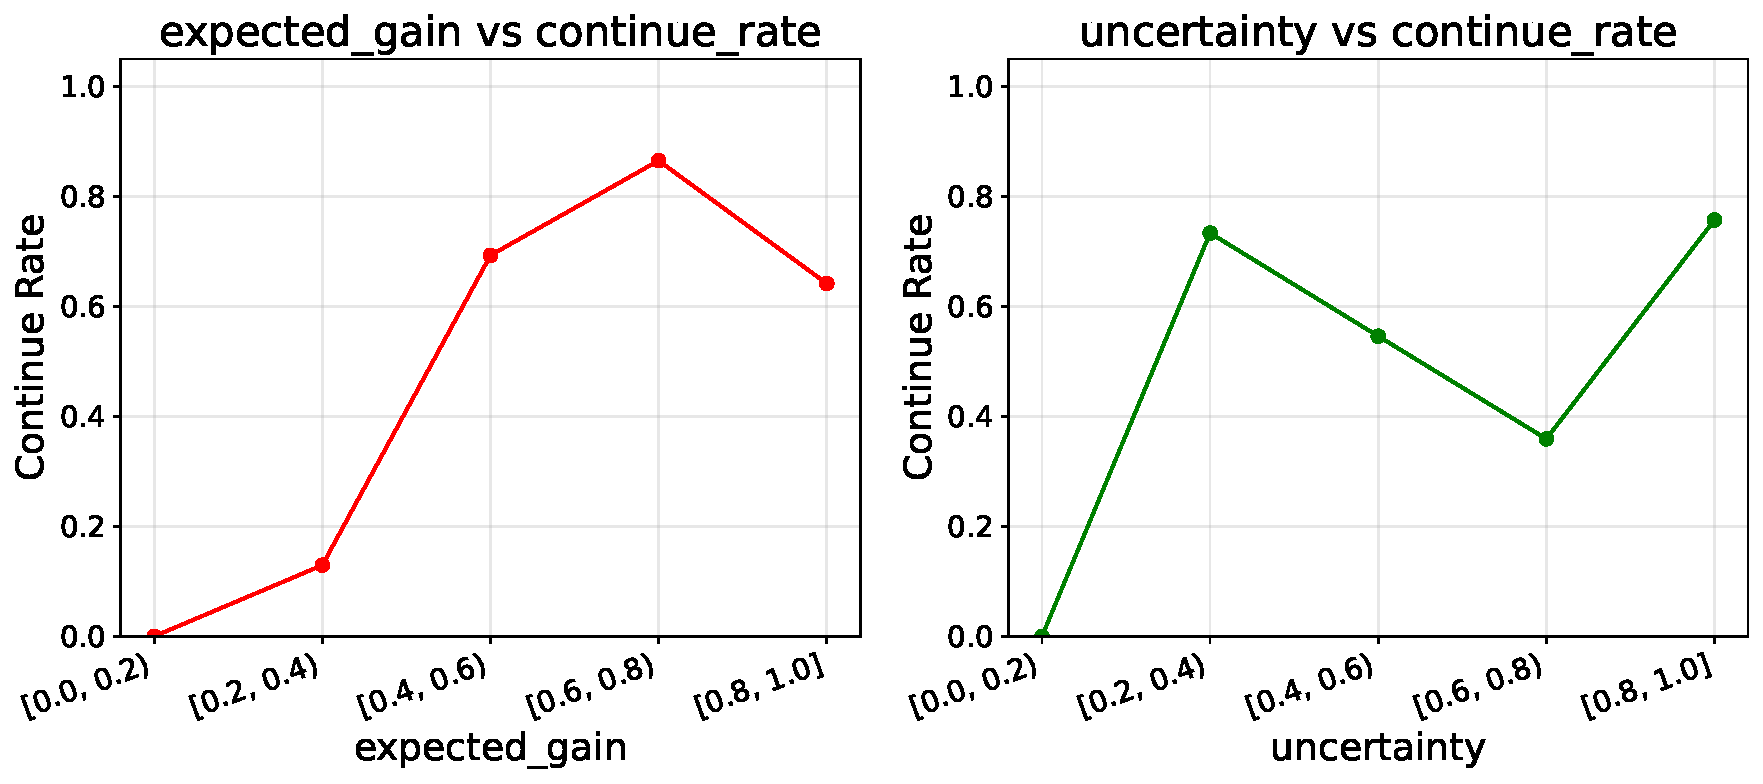
\includegraphics[width=0.92\linewidth]{figures/figure6_heuristic_signals.pdf}
    \caption{Relationship between heuristic signals and continuation behavior. Continue-rate is much lower in low expected-gain buckets and substantially higher in mid/high-gain buckets, supporting the interpretation of these signals as decision heuristics rather than decorative outputs.}
    \label{fig:heuristic-signals}
\end{figure}

We also inspect whether the internal heuristic signals are behaviorally meaningful. The continue-rate is near zero in the lowest expected-gain bucket, and rises sharply in the mid/high expected-gain range. This is the qualitative pattern we want from a decision heuristic. By contrast, uncertainty is informative but less cleanly monotonic in the current setup. Quantitatively, the Pearson correlation between expected-gain and final F1 is $0.1479$, whereas the correlation for uncertainty is only $0.0131$.

These results support a careful interpretation. We do not present \texttt{expected\_gain} or \texttt{uncertainty} as calibrated probabilities. Rather, they are useful self-estimated control signals whose value lies in shaping action choice and making continuation decisions analyzable.

\subsection{Ablation Analysis}

\begin{figure}[t]
    \centering
    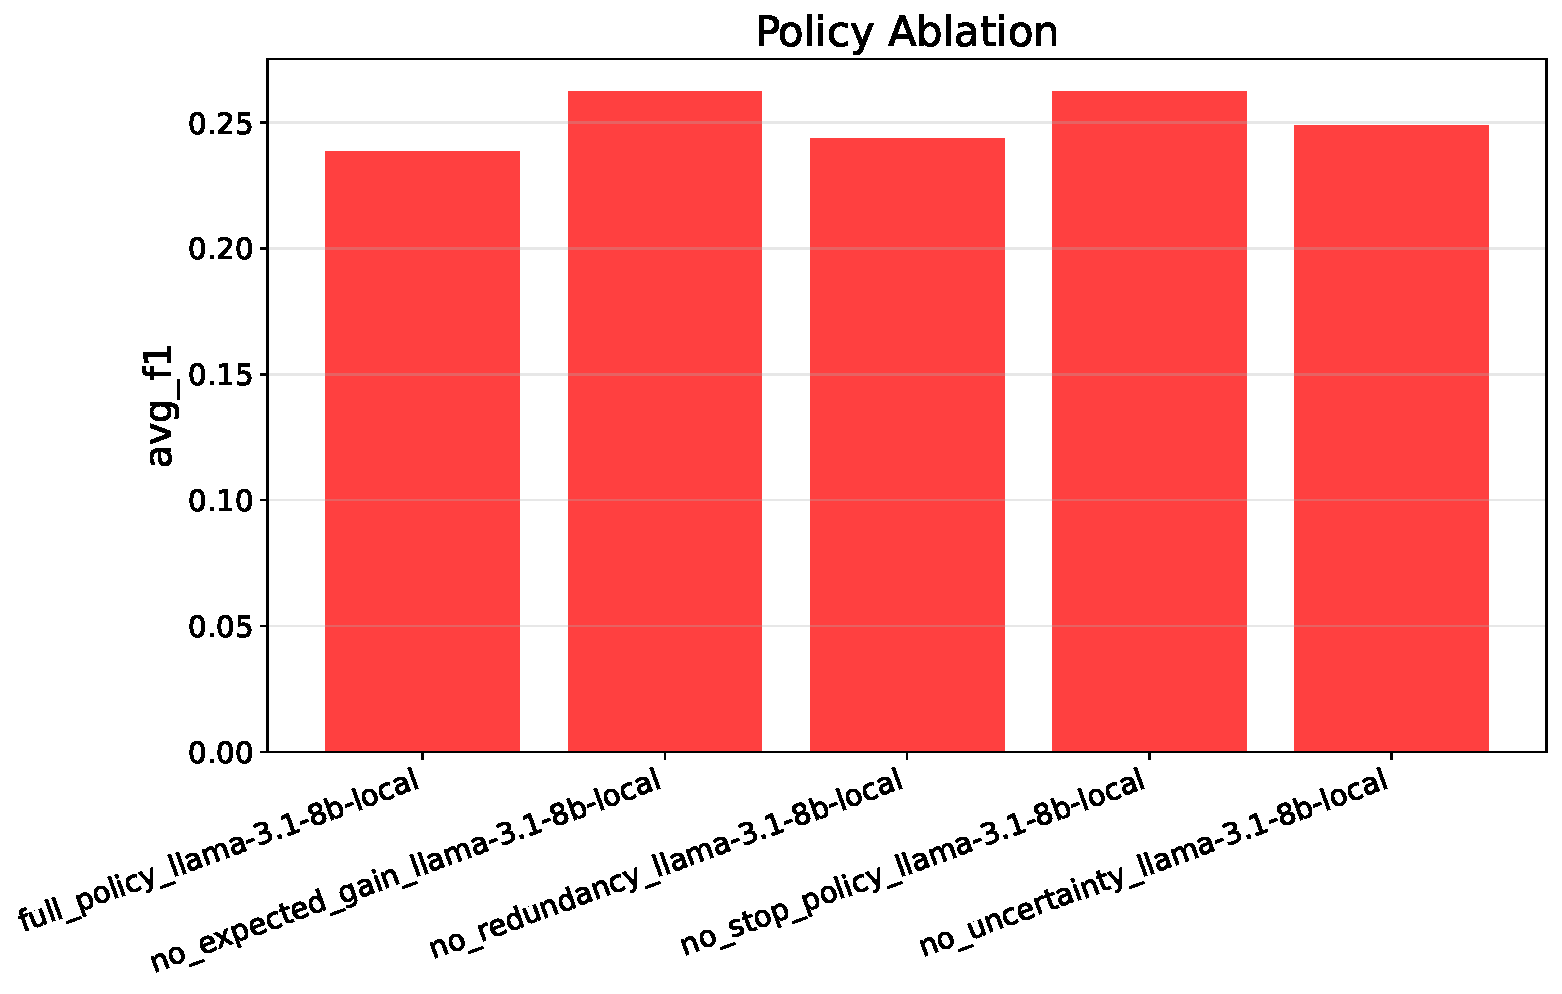
\includegraphics[width=0.80\linewidth]{figures/figure5_policy_ablation.pdf}
    \caption{Policy ablation results. Removing gain-, uncertainty-, redundancy-, or stop-related control generally pushes the agent toward a less favorable quality--cost regime.}
    \label{fig:policy-ablation}
\end{figure}

\begin{table}[t]
\centering
\small
\caption{Policy Ablation}
\begin{tabular}{lrrrr}
\hline
Method & F1 & Tokens & Wall Time & Efficiency \\
\hline
full policy & 0.2383 & 1273.3 & 1.113 & 0.000187 \\
-expected-gain & 0.2621 & 2716.6 & 1.897 & 9.6e-05 \\
-uncertainty & 0.2487 & 1669.7 & 1.378 & 0.000149 \\
-redundancy & 0.2435 & 1792.7 & 1.403 & 0.000136 \\
-stop & 0.2621 & 2716.6 & 1.892 & 9.6e-05 \\
\hline
\end{tabular}
\end{table}


Ablation results reinforce the value of explicit utility components. Figure~\ref{fig:policy-ablation} provides the high-level pattern, while the table gives exact numbers. Removing \texttt{expected\_gain}, uncertainty control, redundancy, or stop-related control generally increases cost more than it improves quality. For example, removing the gain term or stop policy pushes average token usage above $2700$ tokens while only reaching $F1=0.2621$, which is a worse efficiency regime than the full policy. The full policy itself is therefore not the highest-scoring row in absolute terms, but it is the most balanced controlled version.

Overall, the evaluation supports the central claim of the paper: explicit utility-guided orchestration is valuable not only because of final-answer quality, but because it makes the agent's path to that answer controllable, inspectable, and experimentally defensible.

%% --------------------% Discussion %--------------------- %%
\section{Discussion}

Our results suggest that explicit orchestration deserves to be studied as a first-class systems problem for LLM agents. The current literature often emphasizes stronger tools, larger models, or more sophisticated prompting strategies. In contrast, our study highlights that the \emph{control layer} between the model and the environment also plays an important role. Even lightweight utility design can significantly influence how often the agent acts, when it stops, and how much intermediate computation it accumulates.

At the same time, this work has several important limitations. First, the utility components are heuristic rather than learned. Both estimated gain and uncertainty are self-estimated signals, not calibrated probabilities. Second, the current policy is not shown to universally outperform stronger free-form baselines such as ReAct. Our contribution is therefore better understood as a structured orchestration framework and empirical analysis, rather than a universally best-performing method. Third, the current redundancy mechanism improves token compactness more clearly than latency, indicating that better semantic control mechanisms remain an open direction.

These limitations also point to future work. One natural extension is to replace some heuristic signals with learned scorers or calibrated uncertainty estimates. Another is to extend the framework to more complex environments and longer-horizon tasks. It would also be valuable to investigate explicit memory-aware orchestration, where retrieval, memory reading, and memory writing are controlled under the same decision framework. More broadly, our findings support the view that efficient LLM agents require not only strong reasoning models, but also explicit decision policies that constrain and organize multi-step behavior.
%% --------------------% Conclusion %--------------------- %%
\section{Conclusion}

This paper studies tool-using LLM agents from the perspective of explicit orchestration. Rather than relying entirely on fixed workflows or unconstrained prompt-driven reasoning, we formulate agent control as a utility-guided decision process over actions such as responding, retrieving, calling tools, verifying, and stopping. The resulting framework makes it possible to analyze how estimated gain, cost proxies, uncertainty, and redundancy shape the quality--cost trade-off of agent execution.

Our experiments show that explicit utility design provides a practical and defensible way to study agent behavior, even when the underlying signals are heuristic. Additional analyses of cost definitions, workflow fairness, and redundancy control further clarify what the policy is doing and what it is not doing. Overall, the main value of this work is not a claim of universal dominance, but a structured step toward more controllable, analyzable, and cost-aware LLM agents.
We believe this perspective is particularly relevant for budget-sensitive and context-limited deployments, where multi-step agent behavior must be effective not only in quality, but also in cost and control.
%% -----------------% acknowledgements %------------------- %%
%\input{sections/acknowledgements.tex}
%% --------------------% Reference %---------------------- %%
%% Either use w/ the ACM-Reference-Format style (NOTE: my option),
%% or BibLaTeX w/ the acmnumeric or acmauthoryear sytles
\clearpage %DEBUG: 

\bibliographystyle{ACM-Reference-Format}
\bibliography{main}
%% --------------------% Appendix %---------------------- %%
%% If your work has an appendix, this is the place to put it.
%% \appendix
%% \section{Research Methods}
%%
% \begin{appendix}
% \section{Ethics}
% This work does not raise ethical concerns.
% \end{appendix}

\end{document}
\endinput